\documentclass{bioinfo}
\copyrightyear{2012}
\pubyear{2012}

\usepackage{subfig}
\usepackage{listings}
\usepackage{ifthen}
\usepackage[english]{babel}
\usepackage[normalem]{ulem}

\lstset{language=Java,
morendkeywords={String, Throwable}
captionpos=b,
basicstyle=\scriptsize\ttfamily,%\bfseries
stringstyle=\color{darkred}\scriptsize\ttfamily,
keywordstyle=\color{royalblue}\bfseries\ttfamily,
ndkeywordstyle=\color{forrestgreen},
numbers=left,
numberstyle=\scriptsize,
% backgroundcolor=\color{lightgray},
breaklines=true,
tabsize=2,
frame=single,
breakatwhitespace=true,
identifierstyle=\color{black},
% morecomment=[l][\color{forrestgreen}]{//},
% morecomment=[s][\color{lightblue}]{/**}{*/},
% morecomment=[s][\color{forrestgreen}]{/*}{*/},
commentstyle=\ttfamily\itshape\color{forrestgreen}
% framexleftmargin=5mm,
% rulesepcolor=\color{lightgray}
% frameround=ttff
}

% MACROS:

\newcommand{\TODO}[1]{\textcolor{red}{\textbf{#1}}}
\newcommand{\AbstractDESSolver}{\texttt{Abstract\-DES\-Solver}}
\newcommand{\OverdeterminationValidator}{\texttt{Overdetermination\-Validator}}
\newcommand{\SBMLinterpreter}{\texttt{SBML\-interpreter}}
\newcommand{\FirstOrderSolver}{\texttt{First\-Order\-Solver}}
\newcommand{\AbstractIntegrator}{\texttt{AbstractIntegrator}}
\newcommand{\MultiTable}{\texttt{Multi\-Table}}
\newcommand{\Block}{\texttt{Block}}
\newcommand{\jlibsedml}{\texttt{jlibsedml}}

\hyphenation{
  % TODO hypens for regular words
  im-ple-men-ta-tions
  gra-phi-cal
  bench-mark-ed
}

% some nice colors
\definecolor{royalblue}{cmyk}{.93, .79, 0, 0}
\definecolor{lightblue}{cmyk}{.10, .017, 0, 0}
\definecolor{forrestgreen}{cmyk}{.76, 0, .76, .45}
\definecolor{darkred}{rgb}{.7,0,0}
\definecolor{winered}{cmyk}{0,1,0.331,0.502}
\definecolor{lightgray}{gray}{0.97}

\begin{document}
\firstpage{1}

\title[Simulation Core Library]{Simulation Core Library: a Java
library for numerical computation in systems biology}
\author[Dr\"ager \emph{et~al.}]{%
Andreas Dr\"ager\,$^{1,}$\footnote{to whom correspondence should be
addressed}\hspace{.3em},
Roland Keller\,$^{1,}$\dag,
Alexander D\"orr\,$^{1,}$\footnote{authors with equal
contribution}\hspace{.3em},
Akito Tabira\,$^{2}$,
Akira Funahashi\,$^{2}$,
Michael J. Ziller\,$^{3}$,
Richard Adams\,$^{4}$,
Nicolas Rodriguez\,$^{5}$,
Nicolas Le Nov\`{e}re\,$^{5}$,
Hannes Planatscher\,$^{6}$,
Andreas Zell\,$^{1,*}$}
\address{$^{1}$Center for Bioinformatics Tuebingen (ZBIT), University of
Tuebingen, T\"ubingen, Germany,
$^{2}$Keio University, Graduate School of
Science and Technology, Yokohama, Japan, 
$^{3}$Department of Stem Cell and Regenerative Biology, Harvard University,
Cambridge, MA, USA,
$^{4}$SynthSys Edinburgh, CH Waddington Building, University of Edinburgh,
Edinburgh EH9 3JD, UK,
$^{5}$European Bioinformatics Institute, Wellcome Trust Genome Campus, Hinxton,
Cambridge, UK,
$^{6}$Natural and Medical Sciences Institute at the University of Tuebingen,
Reutlingen, Germany}

\history{Received on XXXXX; revised on XXXXX; accepted on XXXXX}

\editor{Associate Editor: XXXXXXX}

\maketitle

\begin{abstract}
\section{Motivation:}
Dynamic simulation of biological phenomena is a the key aspect of
research in systems biology. However, it is often difficult to use available
implementations of numerical methods as a backend for custom-made programs.
\section{Results:}
The Simulation Core Library is a community-driven project that provides a large
collection of numerical solvers and a sophisticated interface hierarchy for the
definition of custom differential equation systems. It is entirely
implemented in Java\texttrademark{} without the necessity to
include any platform-dependent wrappers or libraries, and does not depend on
any commercial licenses.
%, and can be used on every operating system for which a JVM
%is available.
It already includes an efficient and exhaustive implementation of methods to
interpret the content of models encoded in SBML using the JSBML project.
To demonstrate its capabilities, it has been tested with the
entire SBML Test Suite and %also been used to simulate 
all models of BioModels Database.
\section{Availability:}
Source code, binaries, and documentation can be freely obtained under the terms
of the LGPL version~3 from the website
\href{http://sourceforge.net/projects/simulation-core/}{http://sourceforge.net/projects/simulation-core/}.
\section{Contact:}
\href{mailto:simulation-core-development@lists.sourceforge.net}{simulation-core-development@lists.sourceforge.net}
%
%\section{Supplementary information:}
% TODO: Provide additional material
%Supplementary data is available at Bioinformatics online.
\end{abstract}

%%%\vspace{-.25cm}
\section{Introduction}

As part of the movement towards quantitative biology, modeling, 
simulation, and computer analysis of biological networks have become integral
parts of modern biological research. XML-based standard description formats
such as the Systems Biology Markup Language (SBML, \citealt{Hucka2004}) or
CellML \citep{Lloyd2004} enable encoding of biological network models, and
interpret them in terms of a differential equation system, with additional
structures such as discrete events and algebraic equations.
Software libraries for reading and manipulating the content of
these formats are available.
However, a prerequisite for model analysis, simulation, and calibration (e.g., the
estimation of parameter values), is a multiple-purpose and 
efficient numerical solver library that has been designed with the
requirements of biological network models in mind.

Many stand-alone programs providing these features come with
graphical user interfaces.
%\marginpar{I would avoid naming any software here. Such a list can only be
% incomplete and is not necessary} \sout{, for instance, the Virtual Cell \citep{Loew2001}, iBioSim \citep{Myers2009},
%PottersWheel \citep{Maiwald2008}, COPASI \citep{Hoops2006}, SBToolbox2
%\citep{SBT_Schmidt2006}}
%, or the Systems Biology Workbench with Roadrunner (SBW,
%\citealt{Bergmann06}). 
However, the vast majority of the internal solvers for these systems are part of
larger software suites and can therefore not be easily integrated into custom
programs. Some are implemented in programming languages that are either
platform-dependent (e.g., C or C++) and/or require a commercial license (e.g.,
MATLAB\texttrademark{}) for their execution.
%
%The modeling language SBML (Systems Biology Markup Language,
%\citealt{Hucka2003}) constitutes an important \emph{de facto} standard for the
%exchange of biochemical network models.
%SBML defines a set of data structures and provides rules about how to interpret
%and simulate these kinds of models.
%
%Models in systems biology may combine an ordinary differential equation system,
%which is the basis for numerical simulation, with additional elements such as
%rules and events.  These elements further influence the system. 
%For instance,
%an event takes place if a certain trigger condition becomes true. Whenever this
%happens, event assignments may change the values of model components, such as
%parameter values or compartment sizes. Rules can directly assign new values to
%their objectives, e.g., the concentration of a reacting species.
%

%\sout{The SBML ODE Solver Library \citep{Machne2006}, which is written in C,
%and based on the libSBML library \citep{Bornstein2008}, 
%provides such a simulation routine based on the SUNDIALS differential equation
%solver.}
%\marginpar{I would avoid mentioning it here but keep it for the discussion. It
% makes the current work look like a reimplementation in Java}

The Simulation Core Library presented here is a platform-independent,
well-tested alternative.
This generic library is completely decoupled from any graphical user interface
and can therefore easily be integrated into third-party programs.
It comprises several Ordinary Differential Equation (ODE)
solvers and an interpreter for SBML models. It is the first simulation library
based on JSBML \citep{Draeger2011b}. 
% the Java library JSBML 
%
%Secondly, a graphical and command-line user interface that provides
%a connection to the heuristic optimization framework EvA2 \citep{Kron10EvA2}.
% The combination of SBMLsimulator and EvA2 \citep{Kron10EvA2} estimates the values of all parameters with
%respect to given time-series of metabolite or gene expression values. 
%
Furthermore, the Simulation Core Library contains classes to both export
simulation configurations to SED-ML (Simulation Experiment Description Markup Language,
\citealp{Waltemath2011}), and facilitate the re-use and reproduction of these
experiments by executing SED-ML files.

\begin{methods}
\section{Implementation}
\begin{figure}
%\centerline{
%  \subfloat[Solvers.]{
%    \label{fig:Solvers}
%    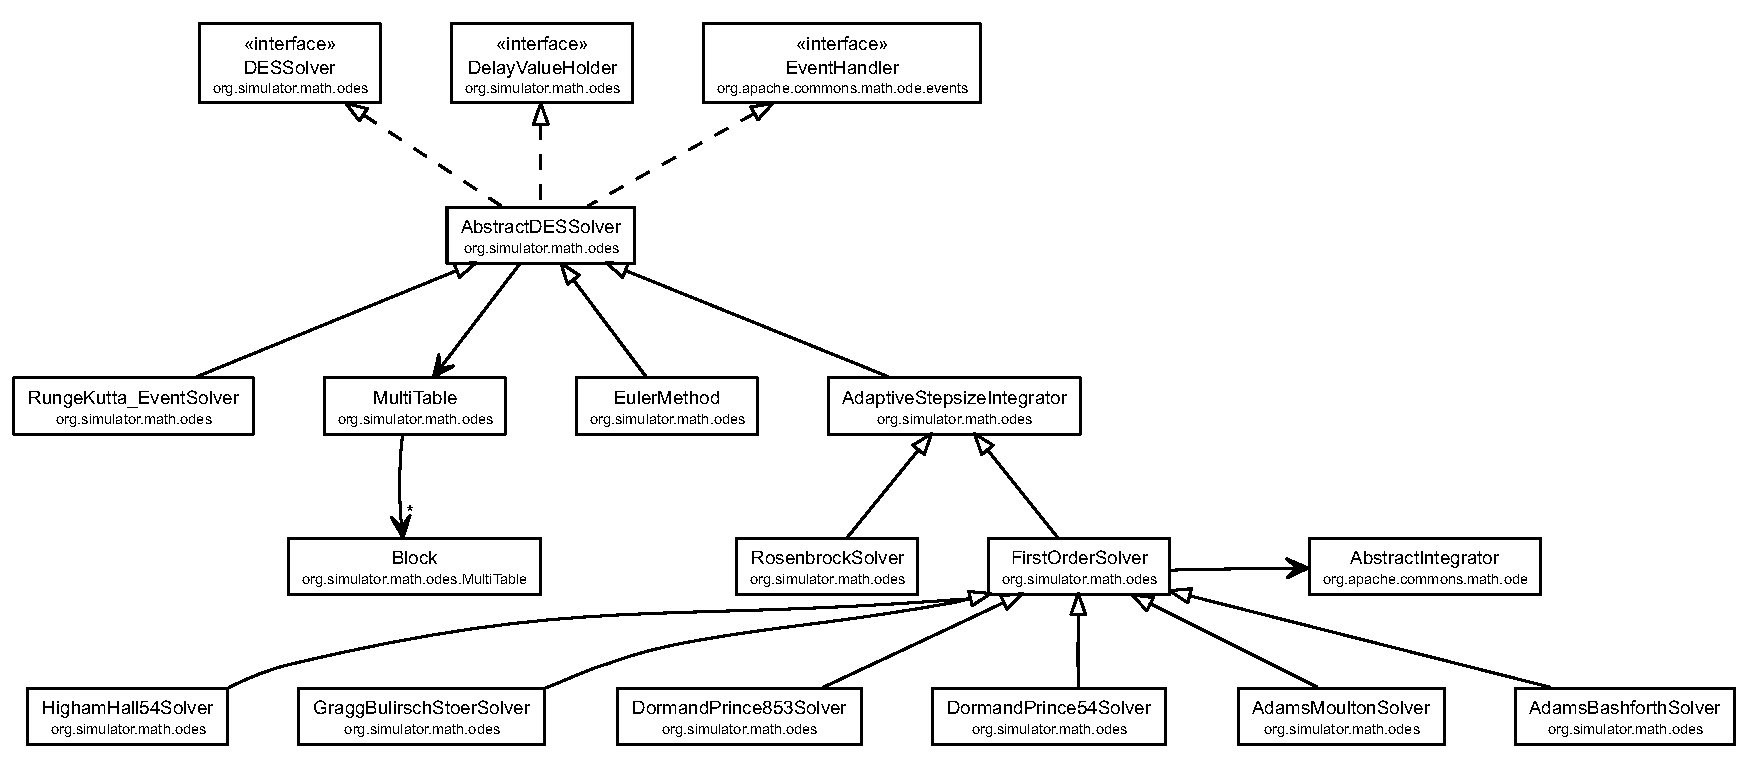
\includegraphics[width=.5\textwidth]{img/Solvers.pdf}
%  }
%  \hfill
%  \subfloat[Differential equation systems.]{
%    \label{fig:DESystems}
%    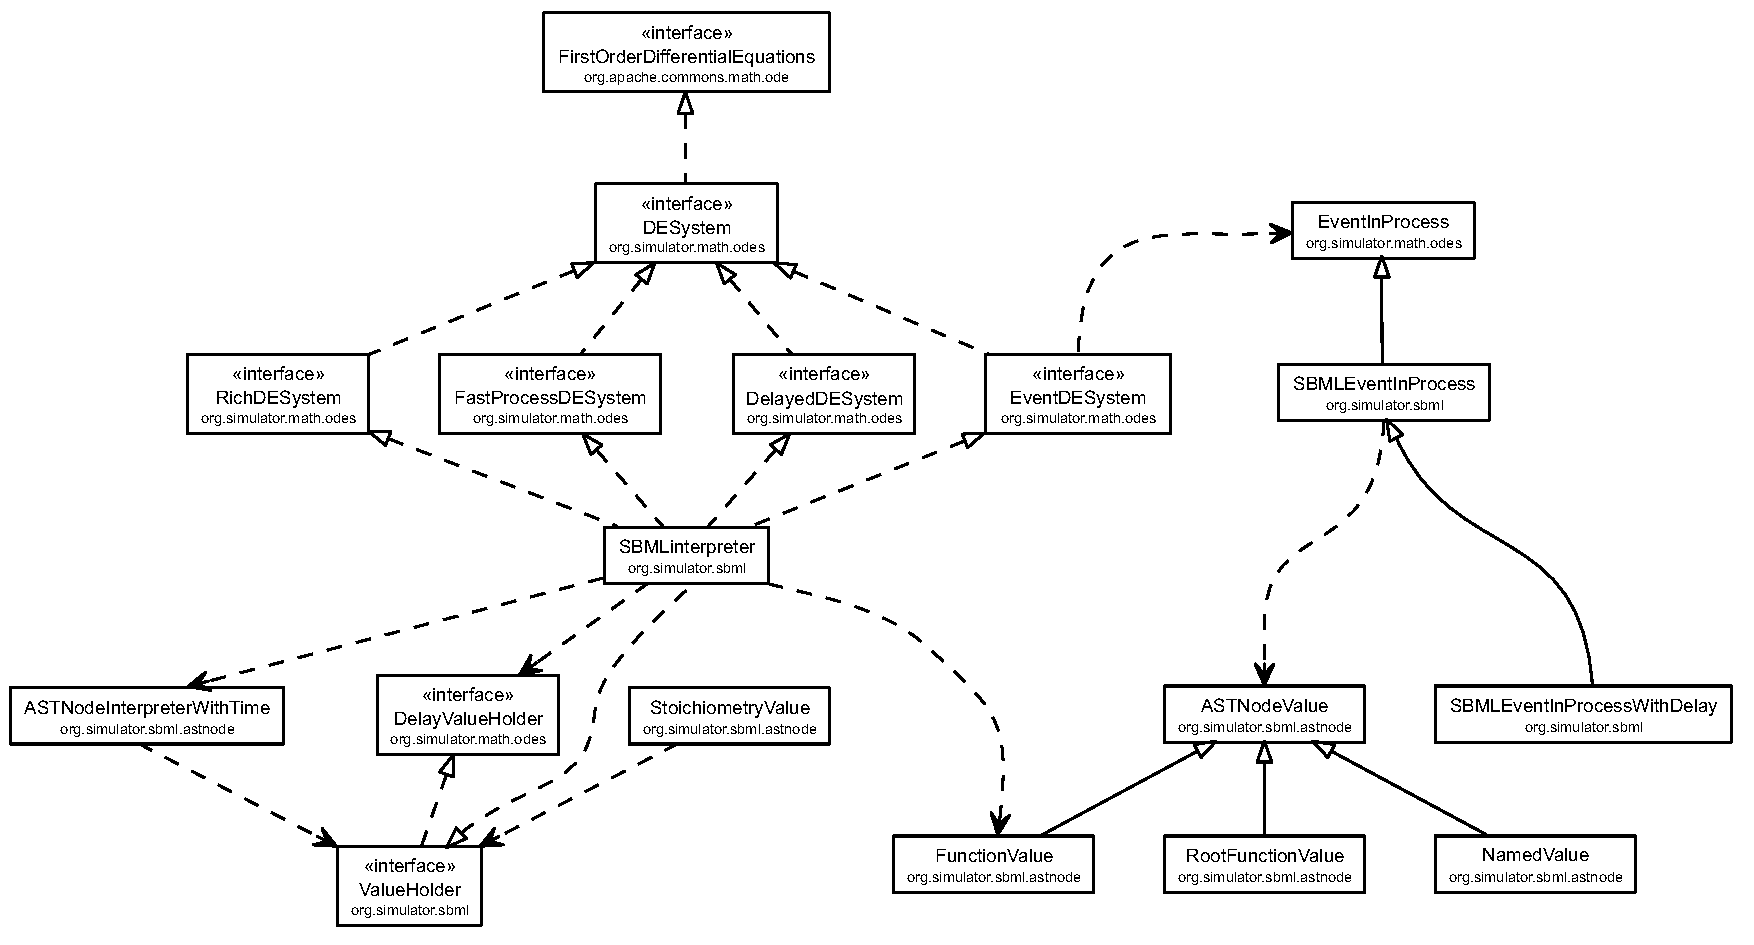
\includegraphics[width=.5\textwidth]{img/SBMLInterpreter.pdf}
%  }
%}
\centering{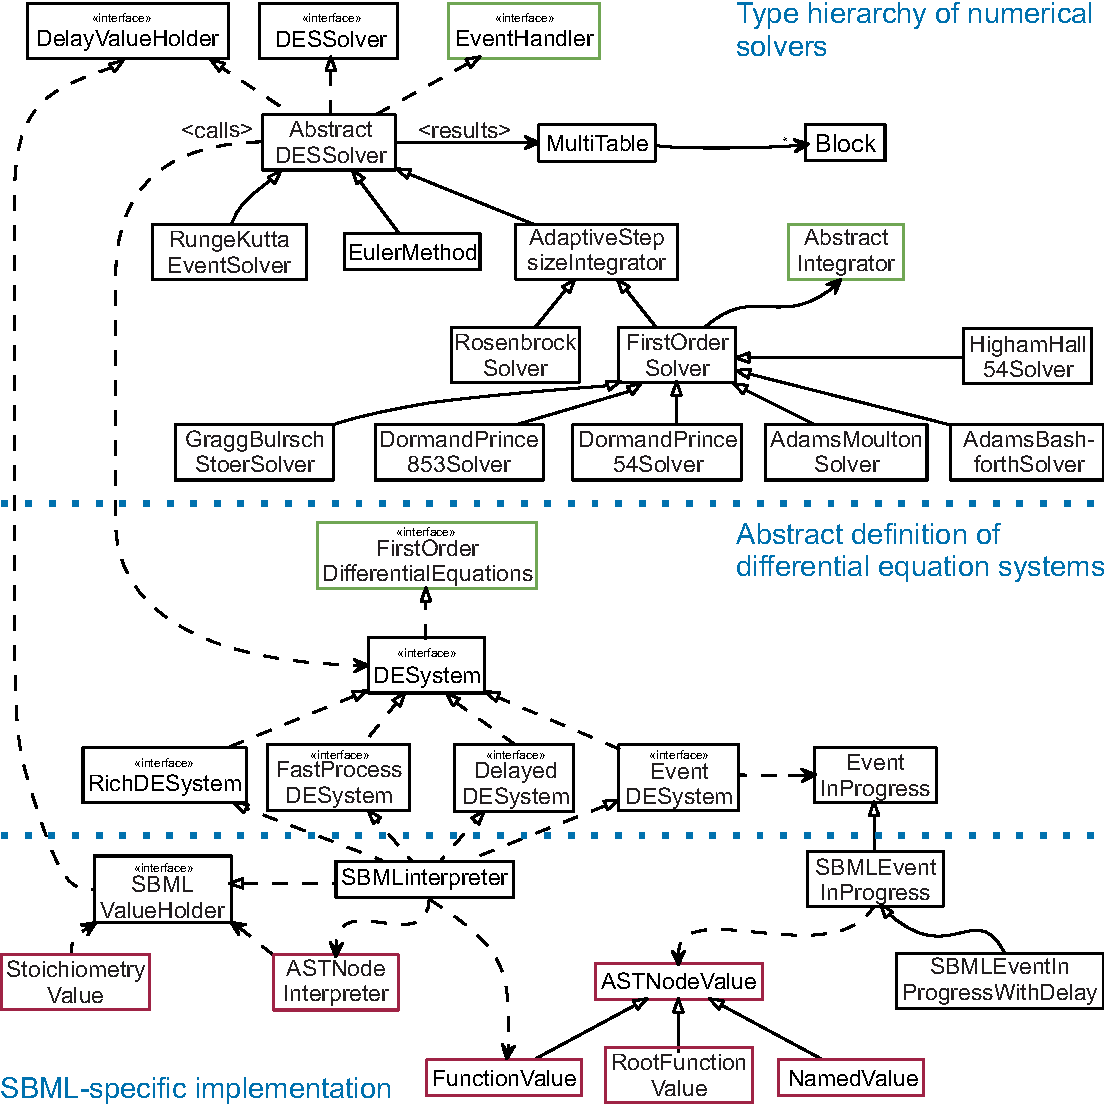
\includegraphics[width=.5\textwidth]{img/UML_Solvers_and_Systems_1.pdf}}
\caption[Architecture of the Simulation Core Library]{Architecture of
the Simulation Core Library (simplified). Numerical methods are
strictly separated from differential equation systems. The upper part displays
the unified type hierarchy of all currently included numerical integration
methods. The middle part shows the interfaces defining several
special types of the differential equations to be solved by the numerical
methods.
The class \SBMLinterpreter{} (bottom part) implements all of these interfaces
with respect to the information content of a given SBML model. Similarly, an
implementation of further data formats can be included into the
library.}%\vspace{-.6cm}}
\label{fig:Architecture}
\end{figure}
All the solver classes are derived from the abstract class \AbstractDESSolver{}
(Fig.~\ref{fig:Architecture}).
Several solvers of the Apache Commons Math library (version 3.0) are integrated
with the help of wrapper classes. Numerical methods and the actual differential
equation systems are strictly separated. The class \MultiTable{} stores the
results of a simulation within its \Block{} data structures. 
%
The abstract description of differential equation systems, with the help of
several distinct interfaces, makes possible to decouple them from a particular
type of biological network. It is therefore possible to pass an instance of an
interpreter for a respective model description format to any available solver.
%\marginpar{I would not quote SBML and CellML. CellML is
% actually not supported at the moment}
%
%A specialized interpreter class is required for the evaluation of a biological
%model. 
This interpretation is the most time consuming step of the integration procedure.
This is why efficient and clearly organized data structures are required to
ensure a high performance of the overall library. The interpretation of SBML
models is split between evaluation of events and rules, computation of
stoichiometric information, and computation of the current values for all model
components (such as species and compartments).
%
For a given state of the ODE system, the class \SBMLinterpreter, responsible
for the evaluation of models encoded in SBML returns the current set of
time-derivatives of the variables.
It is connected to an efficient MathML interpreter of the expressions contained
in kinetic laws, rules and events. The nodes of the syntax tree for those
expressions depend on the current state of the ODE system. If the state has
changed, the values of the nodes have to be recalculated.
At the beginning of the simulation the syntax trees of all kinetic laws, rules
and events are restructured and merged to contain equivalent nodes only once.
This significantly decreases the computation time during the simulation.
%
An important aspect in the interpretation of SBML models is the
determination of the exact time at which an event occurs, as this influences
the precision of the system's variables. We therefore adjusted the Rosenbrock
solver \citep{Kotcon2011}, an integrator with an adaptive step size, to a very
precise timing of the events.
%\sout{Rosenbrock's method is well-suited even for stiff systems.}
%
Algebraic rules are turned into assignment rules before the
simulation: If the system is not overdetermined, exactly one of the variables
contained in an algebraic rule can be chosen as the target variable of the
new assignment rule with the help of a bipartite matching.
%\marginpar{This is only valid for polynomes. And for those,
%assignmentRules should have been used anyway. How do-you proceed for
%cos(x)=0?: Yes, that's true. People should use assignments there, but the
%AlgebraicRules in the test case are all of the type described here. I am
%currently not sure if we could solve cos(x) = 0 or similar cases.}
%
The simulation algorithm then proceeds as follows: For each time step, the ODE
solver gets the current variable values and
calculates the system's state for the next time point. After that, events
and rules are processed, that can change the values. The modified values then
become the initial values for the next time step. The event processing of the
Rosenbrock solver
%\sout{is different from other solvers, as it}
is directly integrated in the solver class and influences the
step size. The time-accurate handling of events and rules leads to very precise
results of the simulation.
%
SED-ML support is enabled by inclusion of the \jlibsedml{} library
(\href{http://www.jlibsedml.org}{http://www.jlibsedml.org}) in the binary
download. Clients of the the Simulation Core Library can choose to use the
\jlibsedml{} API directly, or access SED-ML support via  facade classes
in the \texttt{org.simulator.sedml} package that do not require direct
dependencies on \jlibsedml{} in their code.
\end{methods}

%\begin{table}[!t]
%\processtable{This is table caption\label{Tab:01}}
%{\begin{tabular}{llll}\toprule
%head1 & head2 & head3 & head4\\\midrule
%row1 & row1 & row1 & row1\\
%row4 & row4 & row4 & row4\\\botrule
%\end{tabular}}{This is a footnote}
%\end{table}


%%%%%%%%%%%%%%%%%%%%%%%%%%%%%%%%%%%%%%%%%%%%%%%%%%%%%%%%%%%%%%%%%%%%%%%%%%%%%%%%%%%%%
%
%     please remove the " % " symbol from \centerline{\includegraphics{fig01.eps}}
%     as it may ignore the figures.
%
%%%%%%%%%%%%%%%%%%%%%%%%%%%%%%%%%%%%%%%%%%%%%%%%%%%%%%%%%%%%%%%%%%%%%%%%%%%%%%%%%%%%%%

\section{Results and conclusion}
The SBML implementation has successfully passed the
SBML Test Suite (version 2.0.2).
%(see
%\href{http://sbml.org/Software/SBML_Test_Suite}{http://sbml.org/Software/SBML\_Test\_Suite}):
Furthermore, it solved 99.27\,\% of the models from the
\href{http://biomodels.net}{BioModels.net} database (release 21,
\citealp{Novere2006a}).
Therefore, the Simulation Core Library is an efficient Java tool for the
simulation of differential equation systems used in systems biology. It can be
easily integrated in larger applications. For instance,
CellDesigner version~4.2 \citep{Funahashi2003} already uses it as one of its simulation libraries.
The stand-alone application SBMLsimulator (available at
\href{http://www.cogsys.cs.uni-tuebingen.de/software/SBMLsimulator}{http://www.cogsys.cs.uni-tuebingen.de/software/SBMLsimulator})
provides a convenient graphical user interface for the simulation of SBML
models and uses it as a computational backend.
The abstract class structure of the library supports the integration of
additional model formats, such as CellML, besides its SBML implementation. To
this end, it is only necessary to implement a suitable interpreter class.

%The SBML ODE Solver Library \citep{Machne2006}, which is written in C,
%and based on the libSBML library \citep{Bornstein2008}, 
%provides such a simulation routine based on the SUNDIALS differential equation
%solver.

By including support for the emerging standard SED-ML, we hope to facilitate the
exchange, archival and reproduction of simulation experiments performed using
the Simulation Core Library.

\section*{Acknowledgement}

The authors are grateful to B.~Kotcon, S.~Mesuro, D.~Rozenfeld, A.~Yodpinyanee,
A.~Perez, E.~Doi, R.~Mehlinger, S.~Ehrlich, M.~Hunt, G.~Tucker, P.~Scherpelz,
A.~Becker, E.~Harley, and C.~Moore, Harvey Mudd College, USA, for providing a
Java implementation of Rosenbrock's method, and to Michael T.~Cooling,
University of Auckland, New Zealand, for fruitful discussion.

\paragraph{Funding\textcolon} 
The Federal Ministry of Education and Research (BMBF, Germany) in the project
Virtual Liver (grant number 0315756).

\paragraph{Conflict of Interest\textcolon} none declared.
\vspace{-.05cm}

\begin{thebibliography}{}

\bibitem[Dr\"ager {\em et~al.}(2011)Dr\"ager, Rodriguez, Dumousseau, D\"orr,
  Wrzodek, Le~Nov\`{e}re, Zell, and Hucka]{Draeger2011b}
Dr\"ager, A. \emph{et~al.} (2011).
\newblock {JSBML: a flexible Java library for working with SBML}.
\newblock {\em Bioinformatics\/}, {\bf 27}(15), 2167--2168.

\bibitem[Funahashi {\em et~al.}(2003)Funahashi, Tanimura, Morohashi, and
  Kitano]{Funahashi2003}
Funahashi, A. \emph{et~al.} (2003).
\newblock {CellDesigner: a process diagram editor for gene-regulatory and
  biochemical networks}.
\newblock {\em BioSilico\/}, {\bf 1}(5), 159--162.

\bibitem[Hucka {\em et~al.}(2004)Hucka, Finney, Bornstein, Keating, Shapiro,
  Matthews, Kovitz, Schilstra, Funahashi, Doyle, and Kitano]{Hucka2004}
Hucka, M., \emph{et~al.} (2004).
\newblock {Evolving a lingua franca and associated software infrastructure for
  computational systems biology: the Systems Biology Markup Language (SBML)
  project}.
\newblock {\em Systems Biology, IEE\/}, {\bf 1}(1), 41--53.

\bibitem[Kotcon {\em et~al.}(2011)Kotcon, Mesuro, Rozenfeld, and
  Yodpinyanee]{Kotcon2011}
Kotcon, B. \emph{et~al.}  (2011).
\newblock {\em {Final Report for Community of Ordinary Differential Equations
  Educators}\/}.
\newblock Harvey Mudd College Joint Computer Science and Mathematics Clinic,
  301 Platt Boulevard, Claremont, CA 91711.

\bibitem[Le~Nov{\`e}re {\em et~al.}(2006)Le~Nov{\`e}re, Bornstein, Broicher,
  Courtot, Donizelli, Dharuri, Li, Sauro, Schilstra, Shapiro, Snoep, and
  Hucka]{Novere2006a}
Le~Nov{\`e}re, N. \emph{et~al.} (2006).
\newblock {BioModels Database: a free, centralized database of curated,
  published, quantitative kinetic models of biochemical and cellular systems}.
\newblock {\em Nucleic Acids Res\/}, {\bf 34}, D689--D691.

\bibitem[Lloyd {\em et~al.}(2004)Lloyd, Halstead, and Nielsen]{Lloyd2004}
Lloyd, C.~M. \emph{et~al.}  (2004).
\newblock {CellML: its future, present and past}.
\newblock {\em Prog Biophys Mol Biol\/}, {\bf 85}(2-3), 433--450.

\bibitem[Waltemath {\em et~al.}(2011)Waltemath, Adams, Bergmann, Hucka,
  Kolpakov, Miller, Moraru, Nickerson, Sahle, Snoep, and
  Le~Nov\`{e}re]{Waltemath2011}
Waltemath, D. \emph{et~al.} (2011).
\newblock Reproducible computational biology experiments with SED-ML--the
  Simulation Experiment Description Markup Language.
\newblock {\em BMC Syst Biol\/}, {\bf 5}, 198.

\end{thebibliography}

\end{document}
